\chapter{Fundamentos y Panorama Actual}
\label{ch:fundamentos}
Capítulo dedicado a describir los fundamentos y el panorama actual del trabajo. 

\section{Monitorización de Carga No Intrusiva}
\label{se:MonitorizaciondeCargaNoIntrusiva}
Este concepto fue inventado por George W. Hart, Ed Kern y Fred Schweppe en el Instituto Tecnológico de Massachussets, en los años ochenta \autocite{192069}. Fundados por el Electric Power Research Institute, podemos encontrar el proceso básico descrito en la patente estadounidense 4,858,141.

Una breve bibliografía de George W. Hart: Actualmente ejerce como escultor desde 2017. Tiene esculturas en exposición en Berkeley, Princeton, Cambridge, Duke, Brown... Cofundó el Museo de las Matemáticas y se ha retirado recientemente, trabajó en ciencia computacional, matemáticas, educación e investigación.

\subsection{Modelado y Teoría}
\label{sse:ModeladoyTeoria}
La técnica, descrita por Hart, Kern y Schweppe en su publicación modela los consumos en lo que nombran como "Modelo Total de Carga". El modelo total de carga depende de que dispositivos estén encendidos en un momento dado. Por lo que definen un 'proceso de cambio'
$a(t)$ donde a es un dispositivo de consumo eléctrico en un instante de tiempo $t$. Suponiendo $n$ dispositivos,$a(t)$ será un vector Booleano de $n$ componentes:

$$
a_i(t)=
	\left\{
	\begin{array}{l}
	1,\text{si dispositivo } i \text{ encendido en } t\\
	0, \text{si dispositivo } i \text{ apagado en } t
	\end{array}
	\right.
$$

Continúan modelando el sistema de potencia total $P(t)$ para un sistema de corriente alterna como el estado de un dispositivo $a_i$ por su consumo $P_i$ con un pequeño ruido o error $e$
$$
P(t)=\sum_{i=1}^{n} a_i(t)P_i+e(t)
$$

El criterio para determinar el valor de cada una de los dispositivos es entonces:
$$
\hat{a}(t) = \underset{a}{\text{arg min}} \left| P(t) - \sum_{i=1}^{n} a_i(t)P_i \right|
$$

Esto nos lleva a un problema computacionalmente imposible de resolver salvo mediante la fuerza bruta\autocite[4]{192069} y poco margen de mejora en el modelado para simplificar su resolución. De manera resumida, el problema trata en encontrar el número de dispositivos y el consumo de cada uno. 
Este es un problema que se beneficia de hacer uso de modelos heurísticos.

El concepto de NILM desde su introducción ha sido el método preferido por ingenieros e investigadores para la disgregación de consumo desde su introducción, debido a sus ventajas económicas y prácticas.\autocite[pág. 2, pár. 4]{Nalmpantis2019}

En cuanto al origen de este método, se buscó categorizar los dispositivos dentro de tres grandes grupos, para poder estructurar los diferentes dispositivos y generalizar el modelado de dispositivos específicos. 
Estos grupos son: 

\begin{enumerate}
\item \textbf{Señales de estados fijos} Siguen la arquitecturea de una máquina de estados finita, las transiciones entre estados son consumos exactos, al igual que los estados
\item \textbf{Señales transitorias} Esto son señales que no se encuentran en un espacio discreto que permita modelar su comportamiento como una máquina de estados. Un ejemplo podría ser un calefactor automático, que regula su generación de calor en función de la diferencia de la temperatura ambiente y la temperatura objetivo.
\item \textbf{Otras} Señales que no pueden categorizarse en ninguno de los dos casos anteriores. Por ejemplo, los cambios de dirección del motor de una lavadora en el proceso de lavado. 
\end{enumerate}

Cabe mencionar que los propios investigadores reconocieron que en el futuro los dispositivos eléctricos que siguiesen un diseño de máquinas de estados perderían precedencia. Ya que habría más 'dispositivos inteligentes'. Actualmente, una calefacción programable o un aire acondicionado programable están al alcance de cualquiera.
En 2021, en España el 50\% de las viviendas en alquiler constan de aire acondicionado\autocite{idealista2021}. 

Y esto es sólo un dispositivo. Habrá cientos de modelos de cada dispositivo, decenas de marcas, cada dispositivo con sus características específicas. 
Un modelado exhaustivo sería prácticamente imposible de crear y mantener, ya que sólo para el mercado doméstico hay una cantidad desorbitante de dispositivos, combinaciones de dispositivos, ect.

\subsubsection{Un ejemplo de sistema NILM}
Un sistema NILM consta de las siguientes partes: Una fuente de datos (acometida principal). Un dispositivo de recogida de datos (puede ser de Potencia Activa Y reactiva, Voltaje e Intensidad, ect). El modelo predictivo. Y el sistema de consulta de datos, que se ha omitido en la Figura \ref{diagramaNILM}.
\begin{figure}
    \centering
    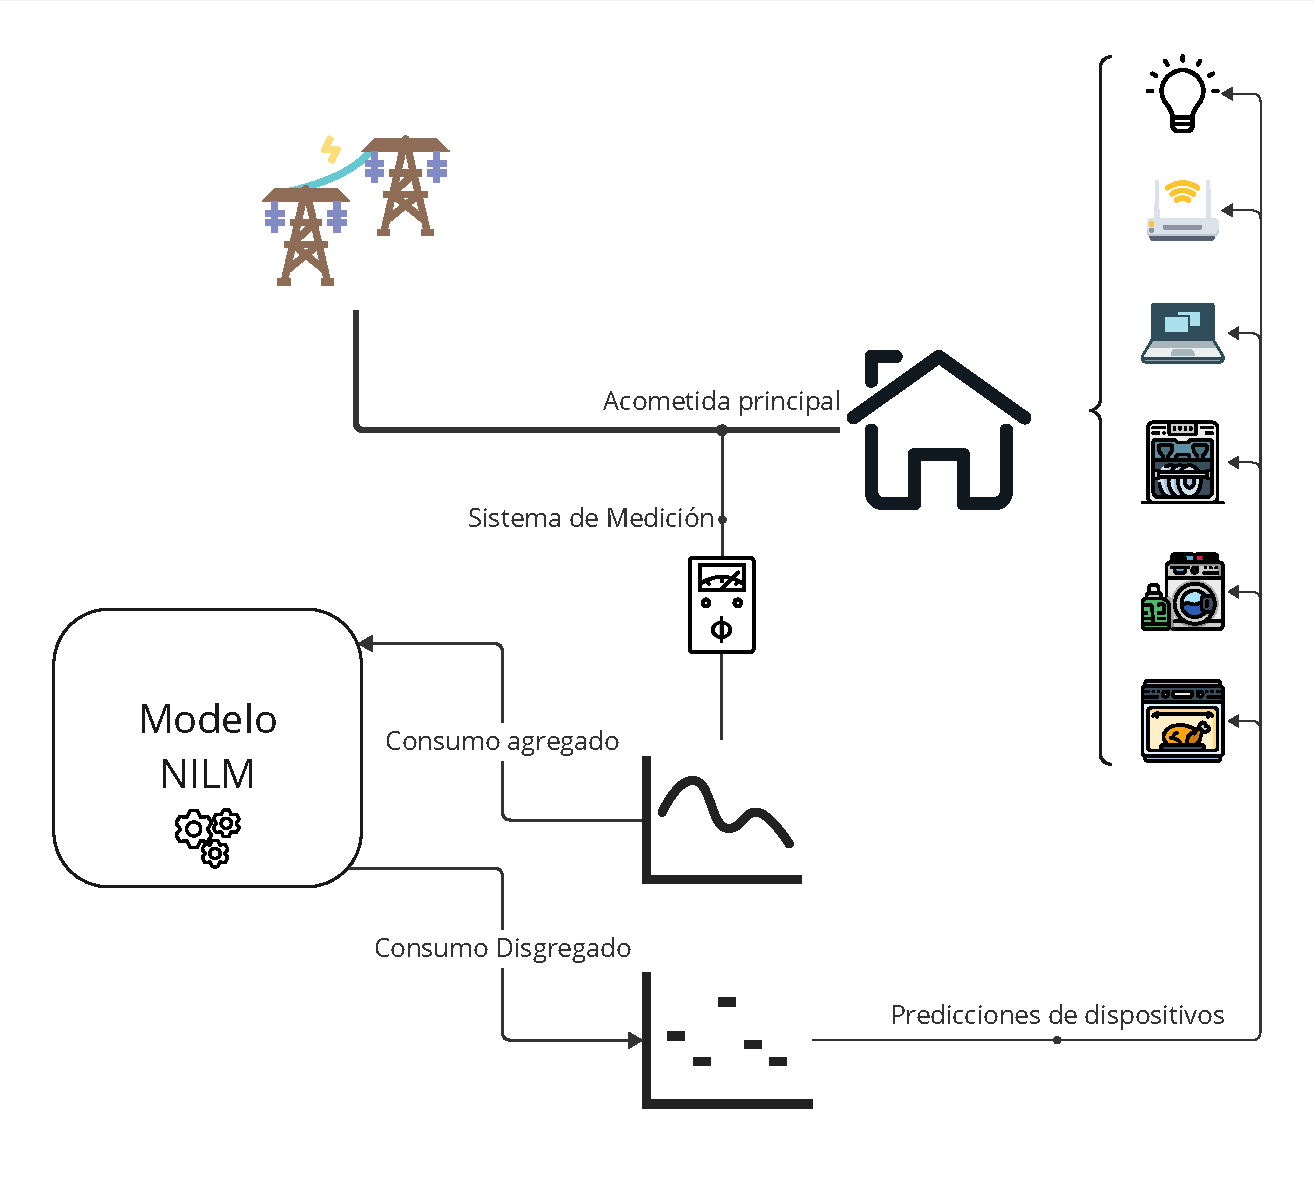
\includegraphics[width=450px]{images/SistemaNILM.pdf}
    \caption{Un diagrama simple de un sistema NILM}
    \label{diagramaNILM}
\end{figure}

Debido a estos argumentos, la investigación de la monitorización no intrusiva se inclinó a los modelos heurísiticos. De los que voy a destacar los Modelos Ocultos de Markov, el Sparse Coding y finalmente las Redes Neuronales. Siendo estas últimas el foco principal del trabajo, y de este capítulo. 

\section{Modelos Ocultos de Markov}
Si se sabe la teoría detrás de una cadena de markov, los modelos de Markov Ocultos resultan una dirección intuitiva a tomar, ya que estos representan la probabilidad de transición de un estado a otro. En esta subsección daremos una breve introducción a la teoría detrás de este modelo probabilístico.
\subsubsection{La Cadena de Markov}
Formalmente, una cadena de Markov se representa por los siguientes componentes:
\begin{center}
    \begin{itemize}
        \item Un conjunto $Q$ de $N$ estados: $$Q = q_1q_2...q_n$$
        \item Una matriz de probabilidad de transición $A$ donde para cada $a_{ij}$ representando la probabilidad de transicionar desde el estado $j$ al estado $i$. $$A=a_{11}a_{12}...a_{N1}...a_{NN}$$ 
        {\footnotesize Cumpliendo $A$ la propiedad: $\sum_{j=1}^n a_{ij} \forall{i}$}
        \item Una distribución de probabilidad inicial $\pi$ sobre los est
        ados. Siendo $\pi_i$ la probabilidad de que la cadena de Markov comience en el estado $i$. $$\pi=\pi_1,\pi_2, ...,\pi_N$$ 
        {\footnotesize Si un estado $j$ tuviera $\pi_j=0$ no podría ser un estado inicial (teniendo probabilidad $0$).\linebreak Además,$\pi$ debe cumplir $\sum_{i=1}^N \pi_i = 1$}
    \end{itemize} 
    \autocite{markovStandford}
\end{center}


\subsubsection{Identificando Datos Ocultos Con Cadenas de Markov}
Una cadena de Markov resulta útil cuando tenemos que modelar un comportamiento en base a una secuencia de eventos observables. 
Estos eventos observables son elementos conocidos, pero la secuencia de estados del modelo para esos eventos observables son desconocidos. 

El problema, como en NILM, es que los estados no son directamente observables. Estan \textit{ocultos} y por tanto debemos ajustar la cadena para incluir una secuencia de posibles similitudes observadas. 

Continuando la explicación de \autocite{markovStandford} en la subsección anterior:
\begin{center}
    \begin{itemize}
        \item Para un elemento $i$ se expresa como $b_i(o)$ donde $o$ es derivado de un conjunto de posibles valores observables $V$.

        \item Dado: $$Q = q_1q_2...q_n$$ 
        \item Calculamos la probabilidad de una cadena de estados $S$ de longitud $T$ $$S=s_1,s_2,...,s_{T}$$
        \item Dado un conjunto de valores observados $$O=o_1,o_2,...,o_{T}$$ para ${T}$ observaciones.
\end{itemize} 
\end{center}

Resumiendo: dados una serie de eventos observables, podemos inferir los estados que causaron estos eventos observables. Calculando la probabilidad de una cadena de eventos observables dada la probabilidad de una cadena de estados del conjunto, para todas las posibles combinaciones de la cadena los estados del conjunto. 
\todo{Texto no definitivo, revisar}

Siendo la fórmula:
$$
\underset{O=o_1,o_2,...,o_{T}}{\text{arg max}} P (O=o_1,o_2,...,o_{T} | S=s_1,s_2,...,s_{T})
$$

Este es el modelado que nos permite inferir de manera probabilística (fórmulas en detalle podrán encontrarse en el \textbf{\autoref{ch:anexob}})\todo{se añadirá el anexo para la entrega de la memoria final}

\subsubsection{Modelos Ocultos de Markov}
Explicadas brevemente las bases de los Modelos Ocultos de Markov, pasamos a la aplicación de este modelo estadístico en la disgregación de consumos.

Dado que un modelo de markov oculto infiere probabilísticamente una serie de estados, esto nos resulta útil para la disgregación de dispositivos. La forma de codificar diferentes estados de diferentes dispositivos se basa aumentando el ancho del modelo. Teniendo una matriz de estados $S_i^j$ donde $S$ es un conjunto de estados. Y las observaciones dependen de todos los estados en un momento dado. Podemos observar esto en el siguiente diagrama:

\begin{center}
    \begin{tikzpicture}
        % Define node styles
        \tikzset{
            latent/.style={circle, draw, minimum size=20pt, inner sep=0pt},
            obs/.style={rectangle, draw, minimum size=20pt, inner sep=0pt},
        }
        
        % Define nodes
        \node[latent] (s1) {$S_{t-1}$};
        \node[latent, right=of s1] (s2) {$S_t$};
        \node[latent, right=of s2] (s3) {$S_{t+1}$};
        \node[obs, below=of s1] (o1) {$Y_{t-1}$};
        \node[obs, below=of s2] (o2) {$Y_t$};
        \node[obs, below=of s3] (o3) {$Y_{t+1}$};
        
        % Connect the nodes with arrows
        \edge[->] (s1) -- (s2);
        \draw[->] (s2) -- (s3);
        \draw[->] (s1) -- (o1);
        \draw[->] (s2) -- (o2);
        \draw[->] (s3) -- (o3);
        \end{tikzpicture}
\end{center}
\todo{pendiente hacer que los vértices aparezcan}%%introducir cita OG
\break
\begin{center}
    \begin{tikzpicture}
        % Define node styles
        \tikzset{latent/.style={circle,draw,minimum size=20pt,inner sep=0pt},
            obs/.style={rectangle,draw,minimum size=20pt,inner sep=0pt},
            e/.style={line,draw, minimum width=2pt}  }
        
        % Define nodes
        \node[latent]                               (s11) {$S_{t-1}^{(1)}$};
        \node[latent, below=of s11]                 (s12) {$S_{t-1}^{(2)}$};
        \node[latent, below=of s12]                 (s13) {$S_{t-1}^{(3)}$};
        
        \node[latent, right=of s11]                 (s21) {$S_t^{(1)}$};
        \node[latent, right=of s12]                 (s22) {$S_t^{(2)}$};
        \node[latent, right=of s13]                 (s23) {$S_t^{(3)}$};
        
        \node[latent, right=of s21]                 (s31) {$S_{t+1}^{(1)}$};
        \node[latent, right=of s22]                 (s32) {$S_{t+1}^{(2)}$};
        \node[latent, right=of s23]                 (s33) {$S_{t+1}^{(3)}$};
        
        \node[obs, below=of s13]                    (o1) {$Y_{t-1}$};
        \node[obs, below=of s23]                     (o2) {$Y_t$};
        \node[obs, below=of s33]                     (o3) {$Y_{t+1}$};
        
        % Connect the nodes
        \edge [e] {s11} {s21} ; %
        \edge [e] {s12} {s22} ; %
        \edge [e] {s13} {s23} ; %
        
        \edge [e] {s21} {s31} ; %
        \edge [e] {s22} {s32} ; %
        \edge [e] {s23} {s33} ; %
        
        \edge [e] {s11,s12,s13} {o1} ; %
        \edge [e] {s21,s22,s23} {o3} ; %
        \edge [e] {s31,s32,s33} {o3} ; %
    \end{tikzpicture}
\end{center}

\todo{pendiente hacer que los vértices aparezcan}%%introducir cita OG

Observando el diagrama b) no resulta muy complicado imaginar la utilidad de este modelo. Si cada cadena representa un dispositivo modelado en diferentes estados, resulta un diseño muy apropiado para NILM.
Los Modelos de Markov Ocultos se han tratado en la literatura como efectivos en comparación con otras técnicas de monitorización cuando el entrenamiento supervisado presenta una baja tasa de muestreo en el eje temporal de la obtención de datos \autocite{frenchHMMNILM}.
Otras ventajas que presenta es su bajo coste computacional en el entrenamiento. Pero el uso de este tipo de elementos lo vuelven altamente susceptible a máximos locales\autocite{NILMreview2017}.

En el caso de los Modelos Factoriales de Markov Ocultos (con siglas FHMM en inglés), presentan ciertas ventajas en comparación con los HMM \footnote{Hidden Markov Models, o en español los Modelos Ocultos de Markov}:
La complejidad y el coste computacional de los los algoritmos de aprendizaje e inferencia son menores para los HMM. Sin embargo, tanto FHMM como HMM presentan limitaciones al volumen máximo de dispositivos simultáneos, incluso en casos como \autocite{afmap2012} donde se propone un nuevo algoritmo no supervisado. El algoritmo desarrollado (AFMAP) no presenta los problemas de alta complejidad y máximos locales, pero requiere de etiquetación manual después de la disgregación. Y presenta bajo rendimiento para dispositivos electrónicos y de cocina \autocite[5]{NILMreview2017}.

\section{Redes Neuronales}
Dado este tercer "verano de la Inteligencia Artificial" . Este tercer verano ocurre en la década de 2010. En 2012 ocurre un avance técnico, unos años antes se creó el reto ImageNet. Un repositorio de más de un millón de imágenes de objetos a lo largo de más de mil categorías diferentes. \autocite{Kautz_2022}
Resulta lógico que el número de artículos científicos proponiendo modelos que permitiesen resolver los retos que presenta NIML aumentase. Y, encontrar

En esta sección se tratan tres conceptos de las Redes Neuronales; se dará una introducción y se expondrán las aplicaciones pertinentes al tema del proyecto.
Por motivos de brevedad, se asume que el lector tiene una cierta base en inteligencia artificial. En caso contrario, sugiero consultar las citas y el \autoref{ch:anexoa}
\subsection{Sparse Coding}
\subsubsection{Breve Introducción}
El Sparse Coding consiste en reducir la activación de la capa oculta de las neuronas, forzando a la red neuronal a realizar un aprendizaje \autocite{stanfordSparse}.
Su objetivo e encontrar un conjunto de vectores $\phi_i$ tal que podamos representar un vector $x$ como una combinación lineal de estos vectores: 
$$
x = \sum_{i=1}^{k}a_i\phi_i
$$
Este es un concepto que está fuertemente relacionado con los autoencoders y el aprendizaje PCA. 

Que tienen como objetivo es que su salida sea igual a la entrada, pero limitando la capa oculta para forzar un aprendizaje. \autocite{stanfordAutoEncoding}
Por ejemplo, supongamos que buscásemos utilizar un autoencoder para comprimir una imagen para enviarla por internet. Si no implementásemos restricciones, dado que el objetivo de la red neuronal es reducir la pérdida de información a 0; la salida del autoencoder sería la imagen, completamente idéntica.
Para evitar esto en el caso de los autoencoders se introduce una capa oculta de menor tamaño en comparación a la capa de entrada como restricción para forzar un aprendizaje, al tener una capa oculta, la capa de salida (de igual tamaño a la de entrada) debe "reconstruir" la entrada \autocite{stanfordAutoEncoding} .

Volviendo al Sparse Coding. Al tener un conjunto de vectores sobrecompleto, los coeficientes $a_i$ ya no se determinan únicamente por el vector de entrada $x$. Luego se define una función de escasez\footnote{De ahí el "Sparse"; escasez en Español}. Definimos esta función de escasez como: tener los menos componentes ($a_i$) distintos de cero o el mínimo de componentes no cerca de cero.

\subsubsection{Aplicaciones}
Tanto los autoencoders como el sparse coding han sido usados en la literatura NILM.
sparse coding:\autocite{SparseCodingNILM}
\todo[inline]{Pendiente continuar investigando}

\subsection{Clasificadores de imágenes}
\subsubsection{Breve Introducción}
\subsubsection{Aplicaciones}

\subsection{Redes Recurrentes}
\subsubsection{Breve Introducción}
\subsubsection{Aplicaciones}

\section{Teoría detrás de la propuesta}
\subsection{Datasets para entrenamiento supervisado en NILM}
\subsection{CSPNet}     
\subsection{Codificación GAF} 
\subsection{Validación de Modelos: NILMTK}  

